
\documentclass[twocolumn, amsmath]{revtex4}

\usepackage{graphicx}
%\graphicspath{ {tex_pics/} }


\begin{document}


\title{PHYS 605 Lab \#7} 

\author{Morgan A. Daly}
\author{Evin O'Shea}
\date{\today} 


\maketitle


\section{Introduction and Theory}
\subsection{Purpose}

The goal of part A of the lab was to investigate the internal resistance of the protoboard's AC voltage supply. This was a good practice in measuring the output voltage and output impedance of a circuit. 

Part A of the lab gave practice for part B of the lab which was to investigate the output impedance of an op amp circuit. In this case the circuit was an inverting amplifier with a gain of three. Along with output impedance, the limitations of possible loads and the affects of differentt resistor values in the op amp circuit.

Part C of the lab was to build a different op amp circuit. The lab group chose to build a high pass filter and amplifier. This circuit's nature was investigated by measuring output voltage versus input frequency. The plot of this relationship will show the nature of the filter.

\subsection{Background / Theory}

Output impedance and voltage of a circuit is important to know. When a voltage is being supplied from an active circuit to a load, the output impedance can tell a lot about the limitations of the loads that can be used. If the output impedance of a passive circuit is much higher than the impedance of the circuit load, then sag can occur. This will mean that the circuit will not work as desired. The magnitude of the output impedance of a circuit can be measured by measuring the ouput voltage of a circuit with no load, and then measuring the ouput voltage with a load. The voltage of the source is measured when the output voltage is measured without the load. When the load is applied, knowing the load resisitance and the voltage across the load will give the current. This information can be used to give the output resistance from the equation:

\begin{equation}
R_{o} =  \frac{V_{R_{o}}}{I_{L}} = (V_{o} - V_{L})\frac{R_{L}}{V_{L}}
\end{equation}

A diagram of the circuit used to make measurements that will allow the norton current to be calculated is shown below:

\begin{figure}[h]
    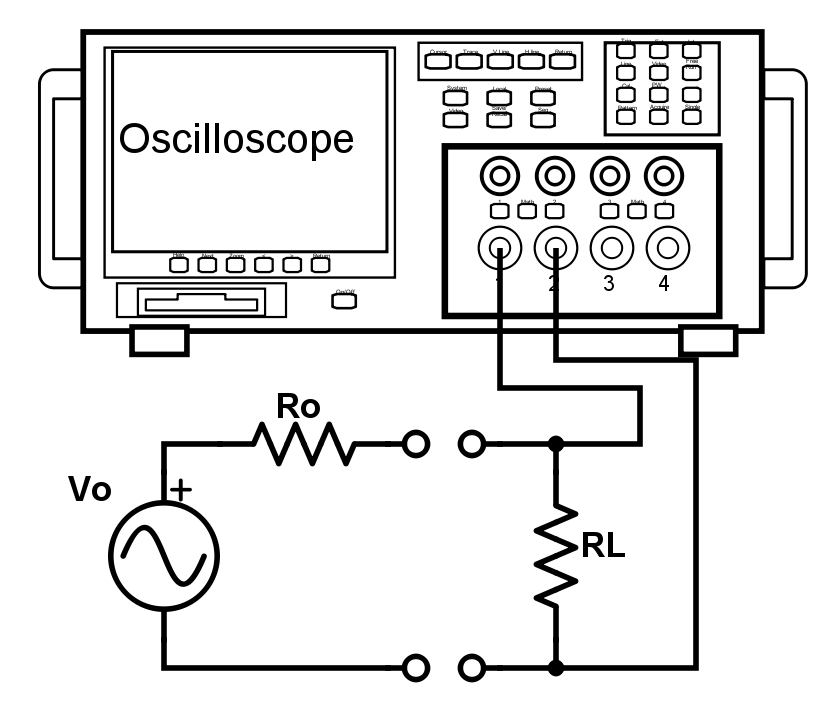
\includegraphics[scale=0.25]{output.png}  
    \caption{This circuit is designed to discover the norton current with can give rise to $R_{o}$ if $V_{o}$ is measured separately.}
\end{figure}

This type of measurement can be made on any circuit. For the second part of the lab, the same set up can be used where $V_{o}$ and $R_{o}$ are the output voltage and output impedance of the circuit created for the second part of the lab.

Op amps are acitve circuit elements that can be used in a multitude of ways. The most important property of an op amp is that the positive and negative terminals of the op amp will be equal. This means that since the positive terminal is grounded, the voltage of the positive and negative terminal will both be zero. This means that $\frac{V_{in}}{R_{in}} = -\frac{V_{out}}{R_{F}}$. Given the definition of the gain we obtain:

\begin{equation}
gain =  \frac{V_{out}}{V_{in}} = -\frac{R_{F}}{R_{in}}
\end{equation}

The invertive amplifier built for this lab is shown below:

\begin{figure}[h]
    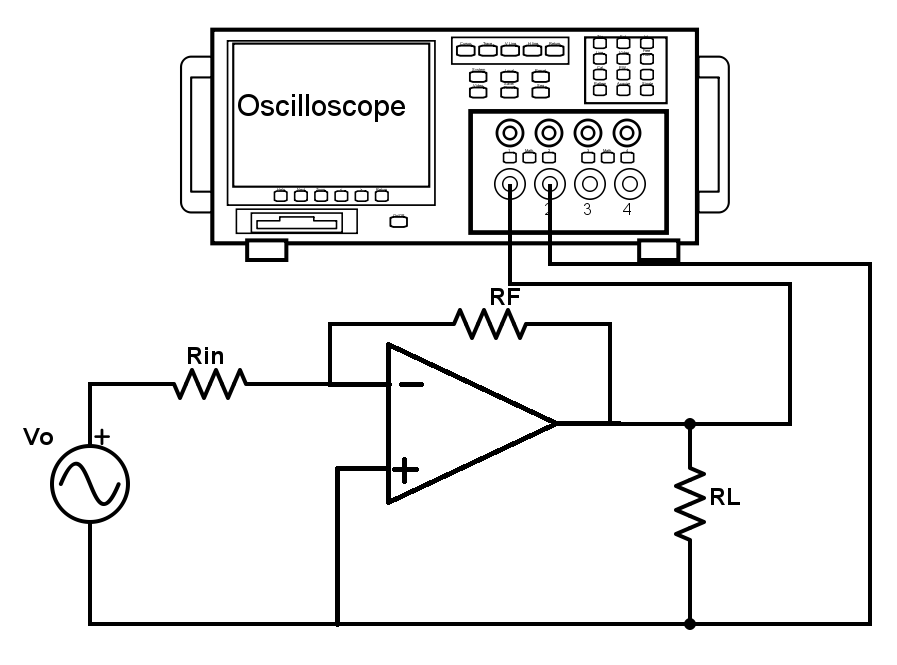
\includegraphics[scale=0.4]{inverting.png}  
    \caption{This circuit is both a high pass filter and an amplifer.}
\end{figure}

For the third part of the lab, a high pass filter and amplifer was made with the op amp. This circuit is shown below. This circuit is a high pass filter because the capacitor only allows high freqency voltages to pass through. In a DC circuit, a capacitor will simply be charged and no current will flow after. In an AC cuircuit, changes in the voltage across the capacitor on one side will cause changes in voltage on the other side. This will allow the AC current to flow through the capacitor. Since the capacitor responds to changes in voltage, higher freqency voltages will pass through the circuit mor easily than low frequency voltages. This is the reason that a circuit in this situation will act as a high pass filter. In this circuit, since there is a negative feedback, the postivie and negative terminals of the op amp will have an equal voiltage. Again, since the positive terminal is grounded, the voltage of the positive and negative terminal will both be zero. Again the gain of this circuit will be determined by:

\begin{equation}
gain =  -\frac{Z_{F}}{Z_{in}}
\end{equation}

This time however, these are complex imedances. In this case, $Z_{in} = R_{in} + C_{in}$. The magnitude of this gain will depend on the frequency of the input voltage. The filter will allow high frequency voltages to pass and low frequencies will have a gain of less than one. The characteristic frequency of an RC circuit is given below:

\begin{equation}
\omega_{RC} =  \frac{1}{R\omega}
\end{equation}

 The op amp circuit built for this part of the lab is shown below:

\begin{figure}[h]
    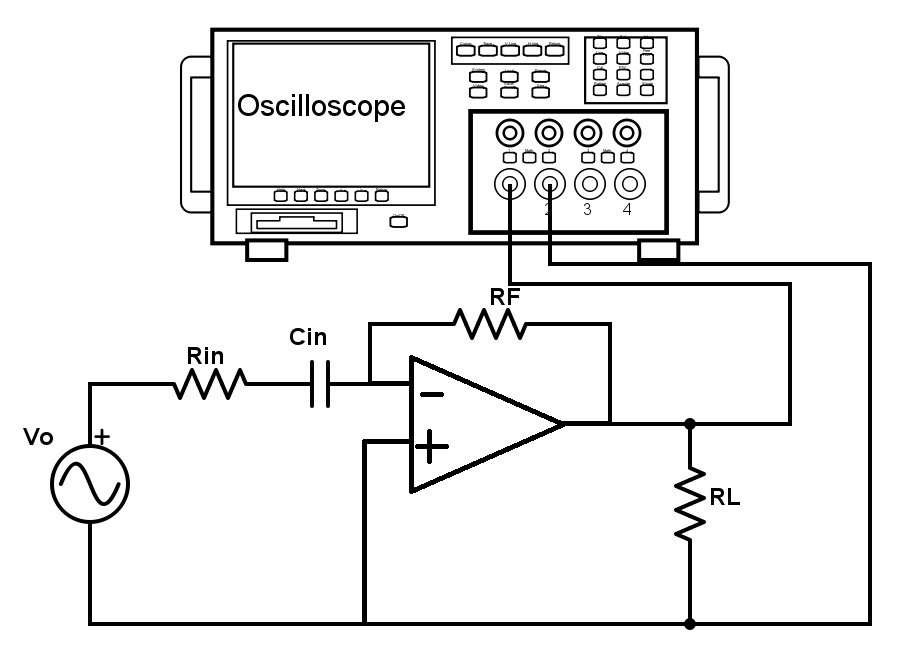
\includegraphics[scale=0.4]{highpassamp.png}  
    \caption{This circuit is both a high pass filter and an amplifer.}
\end{figure}


\section{Methodology}

\begin{enumerate}
    \item Connect the oscilloscope directly to the Protoboard AC voltage supply and mneasure the output voltage.
    \item Set up the circuit shown in figure (1) record the voltage across the resistor and record the resistor value
    \item Build the op amp circuit from figure (2).
    \item Take record of the output voltage with no load attatched.
    \item Add a load to the circuit with a large value as to emilinate sag.
    \item Measure the voltage across the load resistor and the value of this resistor.
    \item Change the frequency and take nots on any changes in the plot on the oscilloscope.
    \item Change the load resistor and investigate the limitations fo the circuit.
    \item Build the circuit from figure (3).
    \item Take recordings of output voltage as the frequency is varied and the input voltage is kept constant.
\end{enumerate}


\section{Results and Analysis}

\subsection{Data}
The goal of part A of the lab was to make measurements to calculate the internal resisitance of the AC voltage source on the protoboard. The data collected for this sectionm is shown below:

\begin{center}
	\begin{ruledtabular}
    \begin{tabular}{ l l l }
	$V_{o}$ (V) & $V_{L}$ (V) & $R_{L}$ (k$\Omega$) \\ \colrule
	3.76 & 3.64 & 22.23  \\
	3.76 & 3.70 & 148.4  \\
	3.76 & 1.04 & 0.2184  \\
	3.76 & 3.68 & 82.1  \\
\end{tabular}
    \end{ruledtabular}
\end{center}

For part C of the lab the group built a high pass filter and amplifier circuit using the op amp. The input voltage used for this section was 1V peak-to-peak. The data recorded is shown below:

\begin{center}
	\begin{ruledtabular}
    \begin{tabular}{ l l }
	frequency (Hz) & $V_{out}$ (V) \\ \colrule
	102000 & 1.76 \\
	92590 & 1.84  \\
	58140 & 1.92 \\
	2119 & 1.88 \\
	1000 & 1.64 \\
	735.3 & 1.46 \\
	457.8 & 1.16 \\
	102 & 0.324 \\
	52.63 & 0.168 \\
	10.75 & 0.044 \\
\end{tabular}
    \end{ruledtabular}
\end{center}


\subsection{Calculations}
The objective of the first part of the lab was to find the internal resistance of the protoboard AC voltage supply. To do this, the group measured the output directly and the output across a load. The group then used equation (1) to obtain the internal resistance of the voltage source.

\begin{center}
	\begin{ruledtabular}
    \begin{tabular}{ l l l }
	$V_{L}$ (V) & $R_{L}$ (k$\Omega$) & $R_{o}$ (k$\Omega$) \\ \colrule
	3.64 & 22.23 & 0.73 \\
	3.70 & 148.4 & 2.41 \\
	1.04 & 0.2184 & 0.571 \\
	3.68 & 82.1 & 1.78 \\
\end{tabular}
    \end{ruledtabular}
\end{center}

From these calculations of $R_{o}$ the average was calculated. $R_{o_{ave}}$ = 1.37k$\Omega$





For Part C of the lab, the gain of the op amp unit is: gain = $\frac{V_{out}}{V_{in}}$ The calculated data for this part of the lab is shown below:

\begin{center}
	\begin{ruledtabular}
    \begin{tabular}{ l l }
	frequency (Hz) & gain (dB) \\ \colrule
	102000 & 4.91 \\
	92590 & 5.30  \\
	58140 & 5.67 \\
	2119 & 5.48 \\
	1000 & 4.30 \\
	735.3 & 3.29 \\
	457.8 & 1.29 \\
	102 & -9.80 \\
	52.63 & -15.5 \\
	10.75 & -27.1 \\
\end{tabular}
    \end{ruledtabular}
\end{center}



\subsection{Analysis}
For part A the group obtained that $R_{o_{ave}}$ = 1.37k$\Omega$. This value is in the range of values obtained. It seems that the protoborad did not have the precsion to accurately measure the voltages to a degree which would allow the calculations to be consistant. With a better measurement device, the data would likely have been more precise.

Part B

For part C of the lab the group built a high pass filter and amplifier circuit using the op amp. For this circuit, a bode plot can be made to shown the nature of the filter. This plot is shown below:

%MORGAN LOOK HERE!!!!!!
\begin{figure}[h]
    \includegraphics[scale=0.4]{bodeplot.png}  
    \caption{}
\end{figure}

At the characteristic frequency, <WRC> the gain is <gain> which is what was expected. The plot demonstrates that the gain in dB is negative for the frequencies below $\omega_{RC}$ and is positive for frequencies above $\omega_{RC}$. This means that the low frequencies are filtered and the high frequencies are passed through the filter. This is the exact nature expected for a high pass filter.

\section{Conclusion}
Part A of the lab was successfully compelte as the internal resistance of the voltage source was calculated. None of the calculated values were very different from the average value. The lab could be improved with a better measurment device for the voltages and by taking more measurements using different load sizes.

Part B 

Part C of the lab was compeleted successfully as the group built an op amp circuit that showed the desired output. The group collected data that showed the nature of the circuit to be a high pass filter.


\end{document}

